\documentclass[aspectratio=169,11pt]{beamer}

\usetheme{Madrid}
\usecolortheme{default}
\usefonttheme{professionalfonts}
\setbeamertemplate{navigation symbols}{}
\setbeamertemplate{footline}[frame number]

\usepackage[T1]{fontenc}
\usepackage{lmodern}
\usepackage{amsmath,amssymb}
\usepackage{graphicx}
\usepackage{booktabs}
\usepackage{xcolor}

% ---------------------------
% Colors
% ---------------------------
\definecolor{myblue}{RGB}{24,84,160}
\definecolor{mydark}{RGB}{34,34,34}
\definecolor{mygray}{RGB}{90,90,90}
\definecolor{mylight}{RGB}{245,247,250}

\setbeamercolor{palette primary}{bg=myblue,fg=white}
\setbeamercolor{palette secondary}{bg=myblue,fg=white}
\setbeamercolor{palette tertiary}{bg=myblue,fg=white}
\setbeamercolor{palette quaternary}{bg=myblue,fg=white}
\setbeamercolor{structure}{fg=myblue}
\setbeamercolor{frametitle}{fg=mydark,bg=white}
\setbeamercolor{title}{fg=mydark}
\setbeamercolor{normal text}{fg=mydark,bg=white}
\setbeamercolor{block title}{bg=myblue!10,fg=mydark}
\setbeamercolor{block body}{bg=mylight,fg=mydark}

% ---------------------------
% Spacing
% ---------------------------
\setlength{\parskip}{0.35em}

% ---------------------------
% Title info
% ---------------------------
\title{Racketlon Match Prediction}
\subtitle{Dynamic Ratings, Machine Learning Models, and Confidence Analysis}
\author{Zain Magdon-Ismail}
\institute{Rensselaer Polytechnic Institute}
\date{}

\begin{document}

% =========================================================
\begin{frame}[plain]
    \titlepage
\end{frame}

% =========================================================
\begin{frame}{Problem}
    \begin{block}{Why is this hard?}
        Racketlon combines four sports---table tennis, badminton, squash, and tennis---into a single total-points competition.
    \end{block}

    \vspace{0.4em}

    \begin{itemize}
        \item Player skill is inherently \textbf{multi-dimensional}
        \item Match outcome depends on both \textbf{sport-level strengths} and \textbf{aggregate scoring}
        \item Performance changes over time, so static skill estimates are not enough
    \end{itemize}

    \vspace{0.5em}

    \textbf{Goal:} predict sport-level score differences, total match score difference, and the final winner.
\end{frame}

% =========================================================
\begin{frame}{Pipeline}
    \begin{center}
        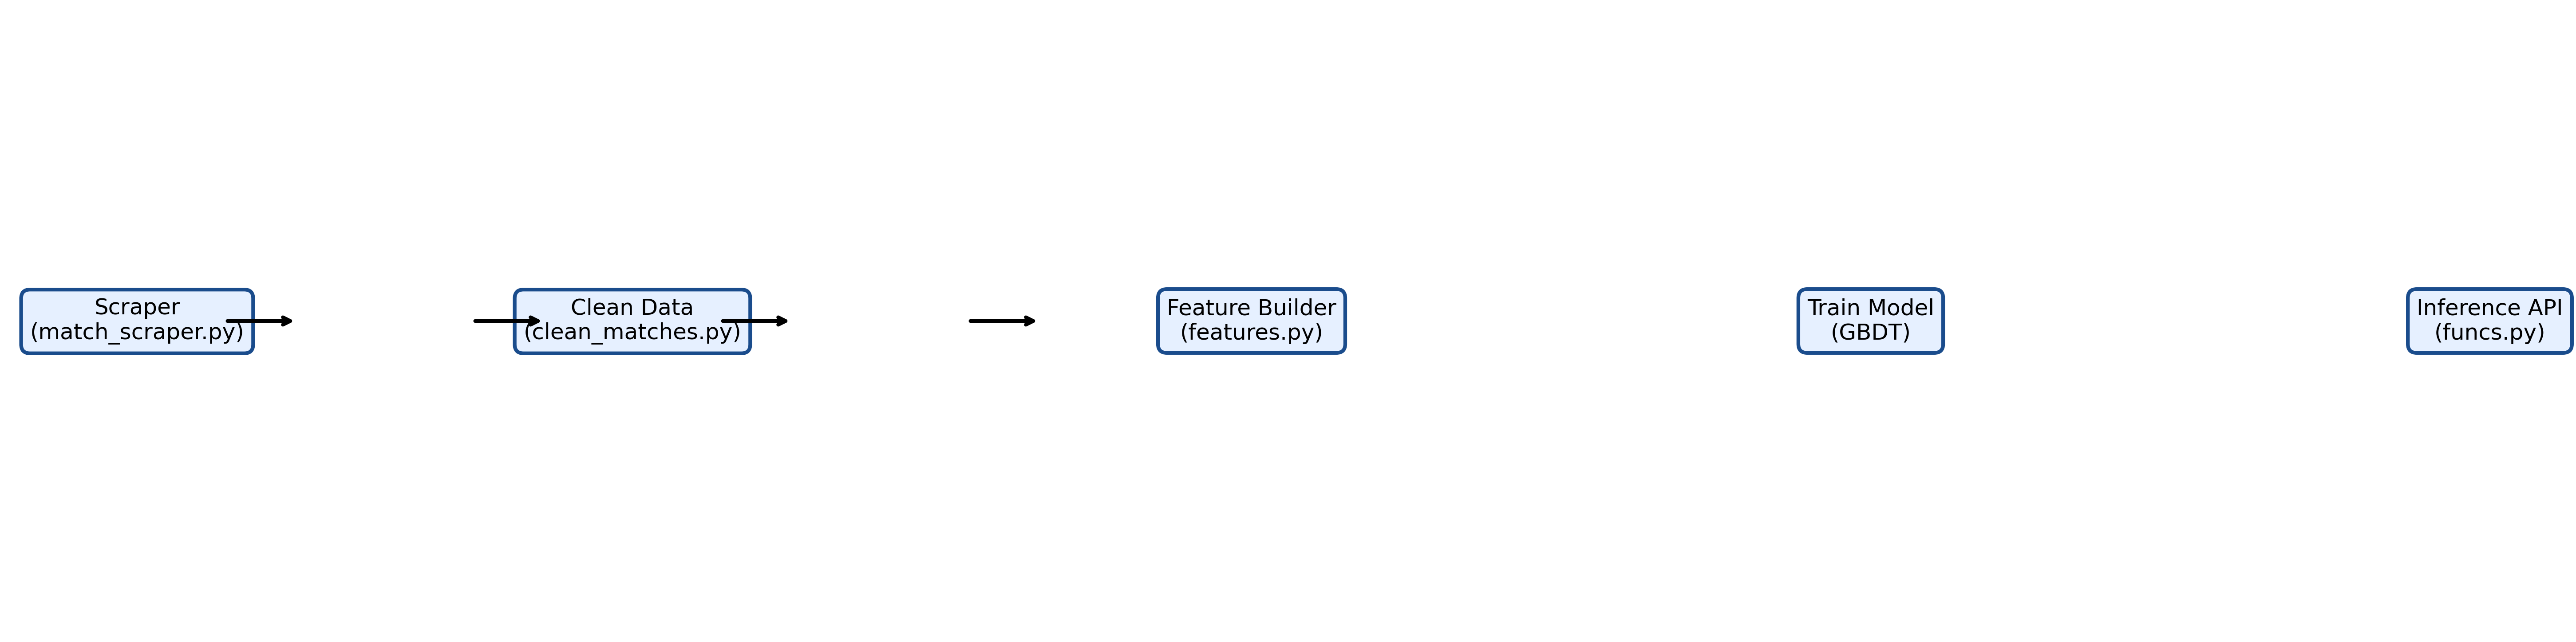
\includegraphics[width=0.82\linewidth]{../poster/poster_images/pipeline.png}
    \end{center}

    \vspace{0.4em}

    \begin{itemize}
        \item scrape historical match data
        \item clean and normalize records
        \item build chronological leakage-safe features
        \item train multiple models
        \item evaluate accuracy and confidence
    \end{itemize}
\end{frame}

% =========================================================
\begin{frame}{Data and Features}
    \begin{columns}[T,onlytextwidth]
        \column{0.52\textwidth}
        \textbf{Data pipeline}
        \begin{itemize}
            \item scraped Tournament Software pages
            \item handled both modern and legacy formats
            \item removed invalid / incomplete matches
            \item normalized player identities
        \end{itemize}

        \column{0.48\textwidth}
        \textbf{Feature groups}
        \begin{itemize}
            \item sport-specific rating differences
            \item recent rolling form
            \item residual performance
            \item long-term averages
            \item head-to-head features
        \end{itemize}
    \end{columns}

    \vspace{0.6em}

    \begin{block}{Important design choice}
        All features were built \textbf{chronologically}, so each match only uses information available before it occurred.
    \end{block}
\end{frame}

% =========================================================
\begin{frame}{Dynamic Rating System}
    For each sport, each player has a separate rating.

    \vspace{0.3em}

    Expected score difference:
    \[
        \hat{d} = 21 \tanh\left(\frac{\alpha (R_1 - R_2)}{2}\right)
    \]

    Experience-dependent learning rate:
    \[
        \eta(g) = \eta_{\min} + (\eta_{\max} - \eta_{\min}) e^{-g/\tau}
    \]

    Time-based adjustment:
    \[
        t_{\mathrm{mult}} = 1 + c_s \left(1 - e^{-d/\tau_s}\right)
    \]

    \vspace{0.4em}

    \begin{itemize}
        \item gives interpretable sport-specific skill estimates
        \item adapts to both experience and inactivity
        \item provides strong predictive features for downstream models
    \end{itemize}
\end{frame}

% =========================================================
\begin{frame}{Models Evaluated}
    \begin{columns}[T,onlytextwidth]
        \column{0.5\textwidth}
        \textbf{Baseline}
        \begin{itemize}
            \item historical average score differences
        \end{itemize}

        \textbf{Linear model}
        \begin{itemize}
            \item ridge regression on engineered features
        \end{itemize}

        \textbf{Player embedding model}
        \begin{itemize}
            \item learned latent player representations
        \end{itemize}

        \column{0.5\textwidth}
        \textbf{Boosted tree model}
        \begin{itemize}
            \item final and strongest model
            \item base prediction + residual correction
        \end{itemize}

        \textbf{Confidence experiment}
        \begin{itemize}
            \item KD-tree neighborhood analysis
            \item tested whether local density predicts reliability
        \end{itemize}
    \end{columns}

    \vspace{0.5em}

    \[
        \hat{d} = b + 0.7r
    \]

    \vspace{-0.2em}
    \centering
    for the final boosted tree differential prediction
\end{frame}

% =========================================================
\begin{frame}{Main Results}
    \begin{block}{Best model: gradient boosted trees}
        \begin{itemize}
            \item match-level MAE: \textbf{8.27}
            \item winner accuracy: \textbf{89\%}
        \end{itemize}
    \end{block}

    \vspace{0.5em}

    \begin{itemize}
        \item baseline was weakest
        \item linear and embedding models improved performance
        \item boosted trees performed best by capturing nonlinear interactions
    \end{itemize}

    \vspace{0.5em}

    \begin{block}{Takeaway}
        Combining a strong rating system with nonlinear machine learning gave the best predictive performance.
    \end{block}
\end{frame}

% =========================================================
\begin{frame}{Prediction Quality}
    \begin{columns}[T,onlytextwidth]
        \column{0.55\textwidth}
        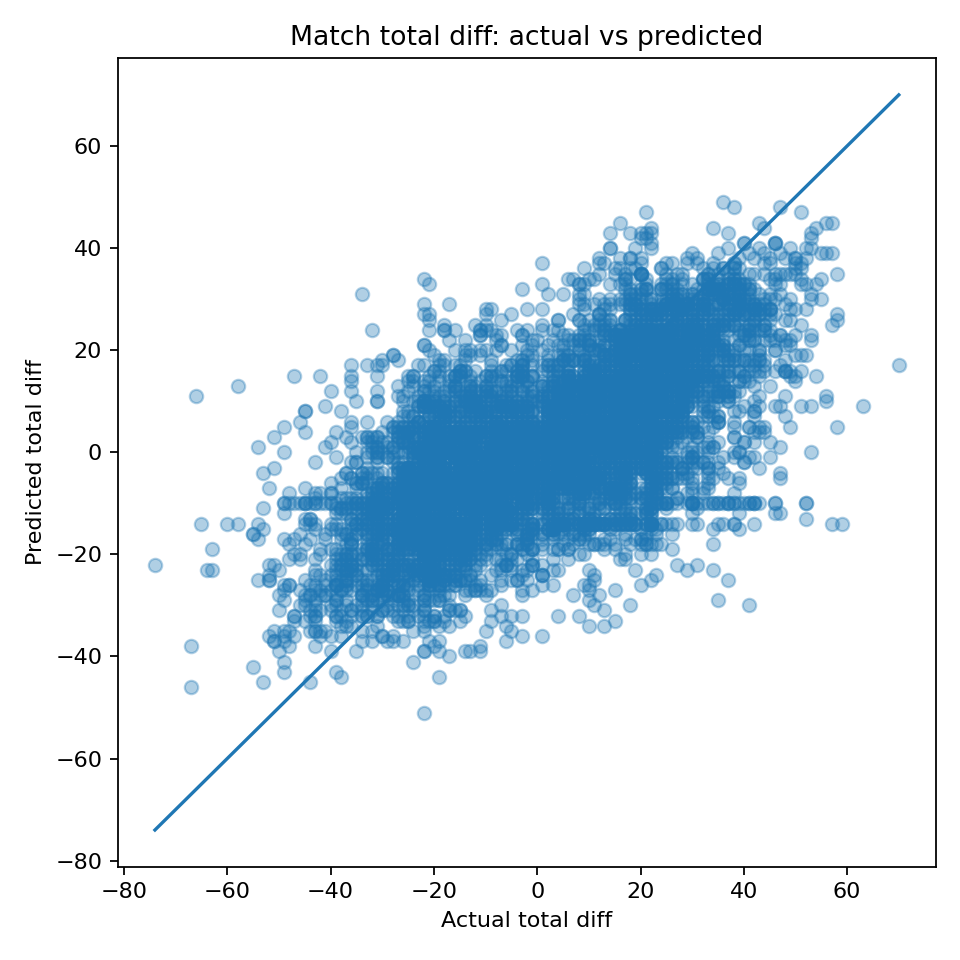
\includegraphics[width=\linewidth]{../paper/figures/match_total_diff_scatter.png}

        \column{0.45\textwidth}
        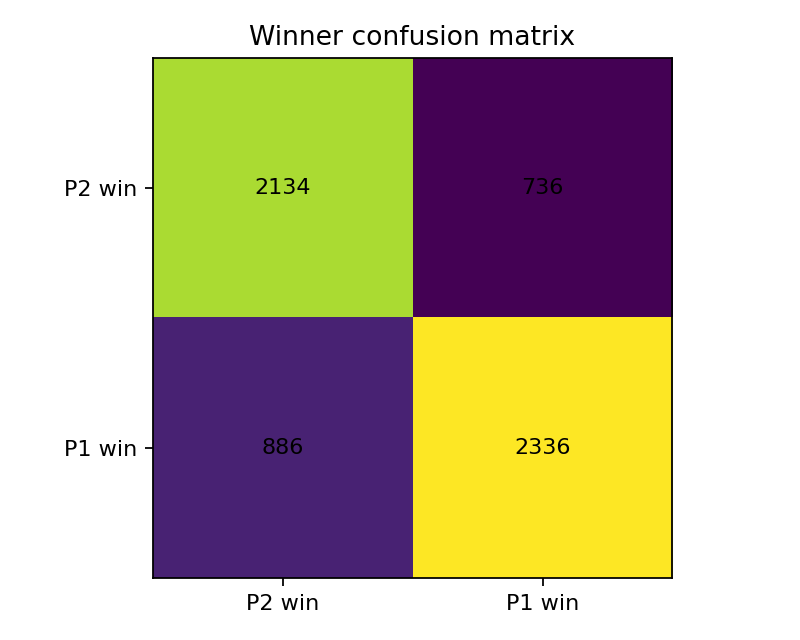
\includegraphics[width=\linewidth]{../paper/figures/winner_confusion_matrix.png}
    \end{columns}

    \vspace{0.5em}

    \begin{itemize}
        \item scatter plot shows the model captures the overall trend in match score difference
        \item confusion matrix shows strong winner classification performance
    \end{itemize}
\end{frame}

% =========================================================
\begin{frame}{Model Comparison and Interpretability}
    \begin{columns}[T,onlytextwidth]
        \column{0.5\textwidth}
        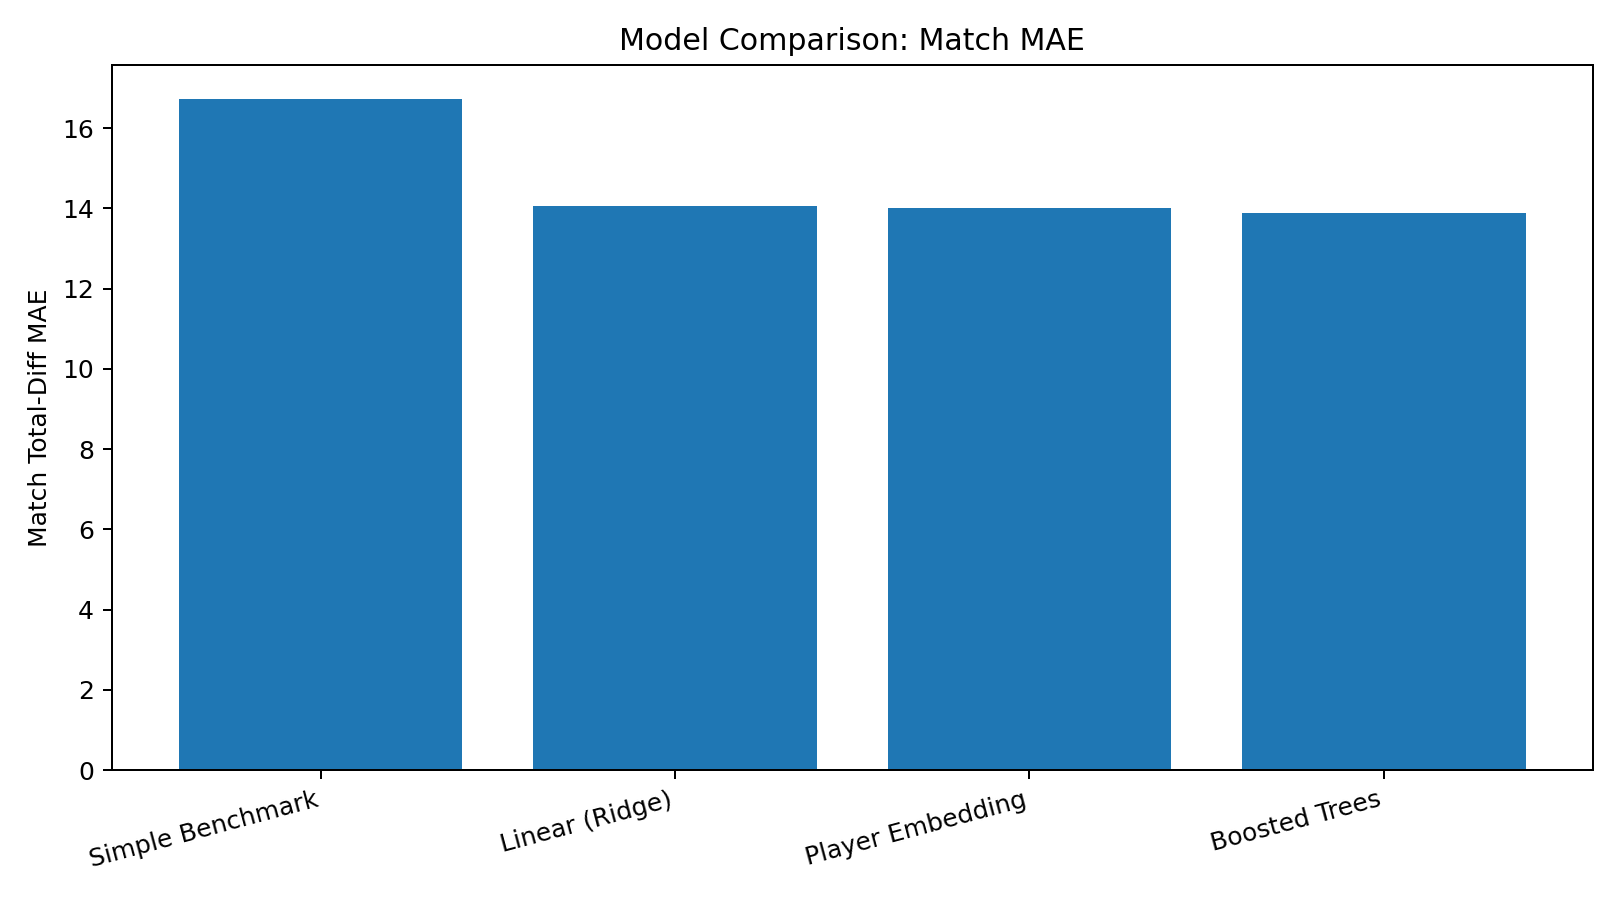
\includegraphics[width=\linewidth]{../paper/figures/model_comparison_mae.png}

        \vspace{0.6em}

        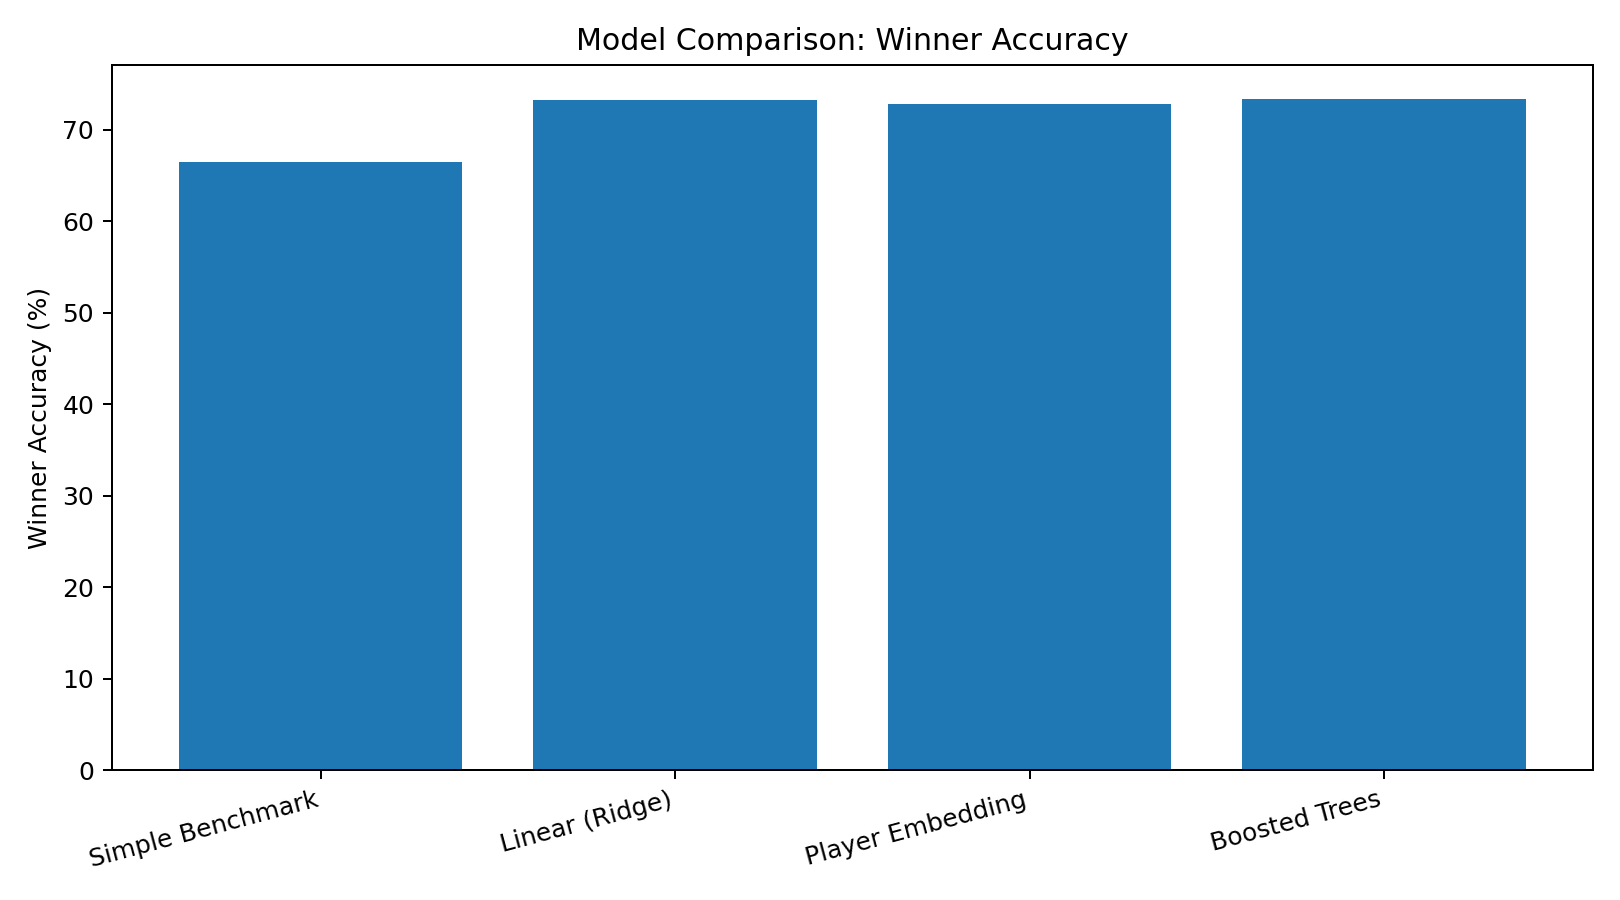
\includegraphics[width=\linewidth]{../paper/figures/model_comparison_accuracy.png}

        \column{0.5\textwidth}
        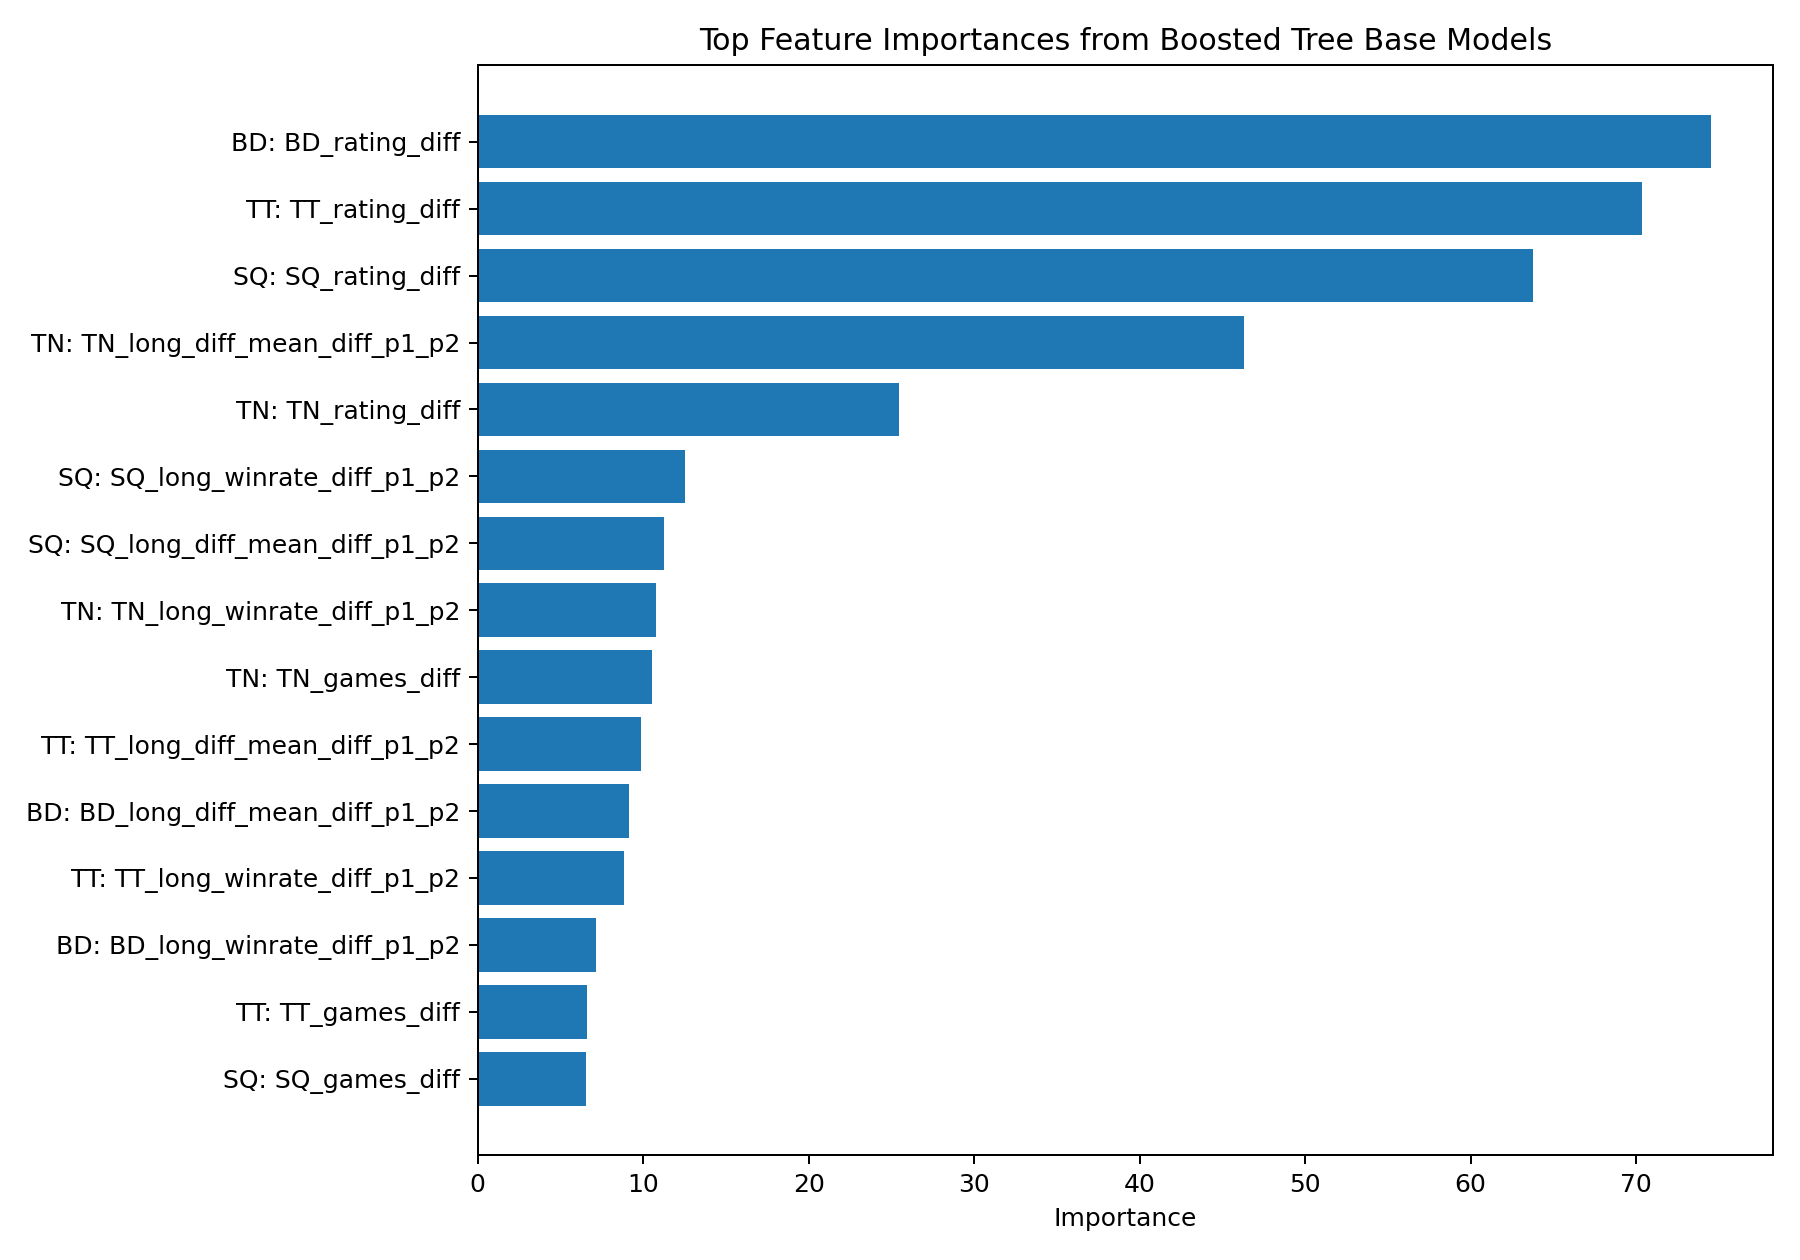
\includegraphics[width=\linewidth]{../paper/figures/feature_importance.png}
    \end{columns}

    \vspace{0.4em}

    \begin{itemize}
        \item nonlinear models outperform simpler baselines
        \item rating-based features dominate the boosted tree model
    \end{itemize}
\end{frame}

% =========================================================
\begin{frame}{Exploratory Confidence Experiment}
    \begin{columns}[T,onlytextwidth]
        \column{0.5\textwidth}
        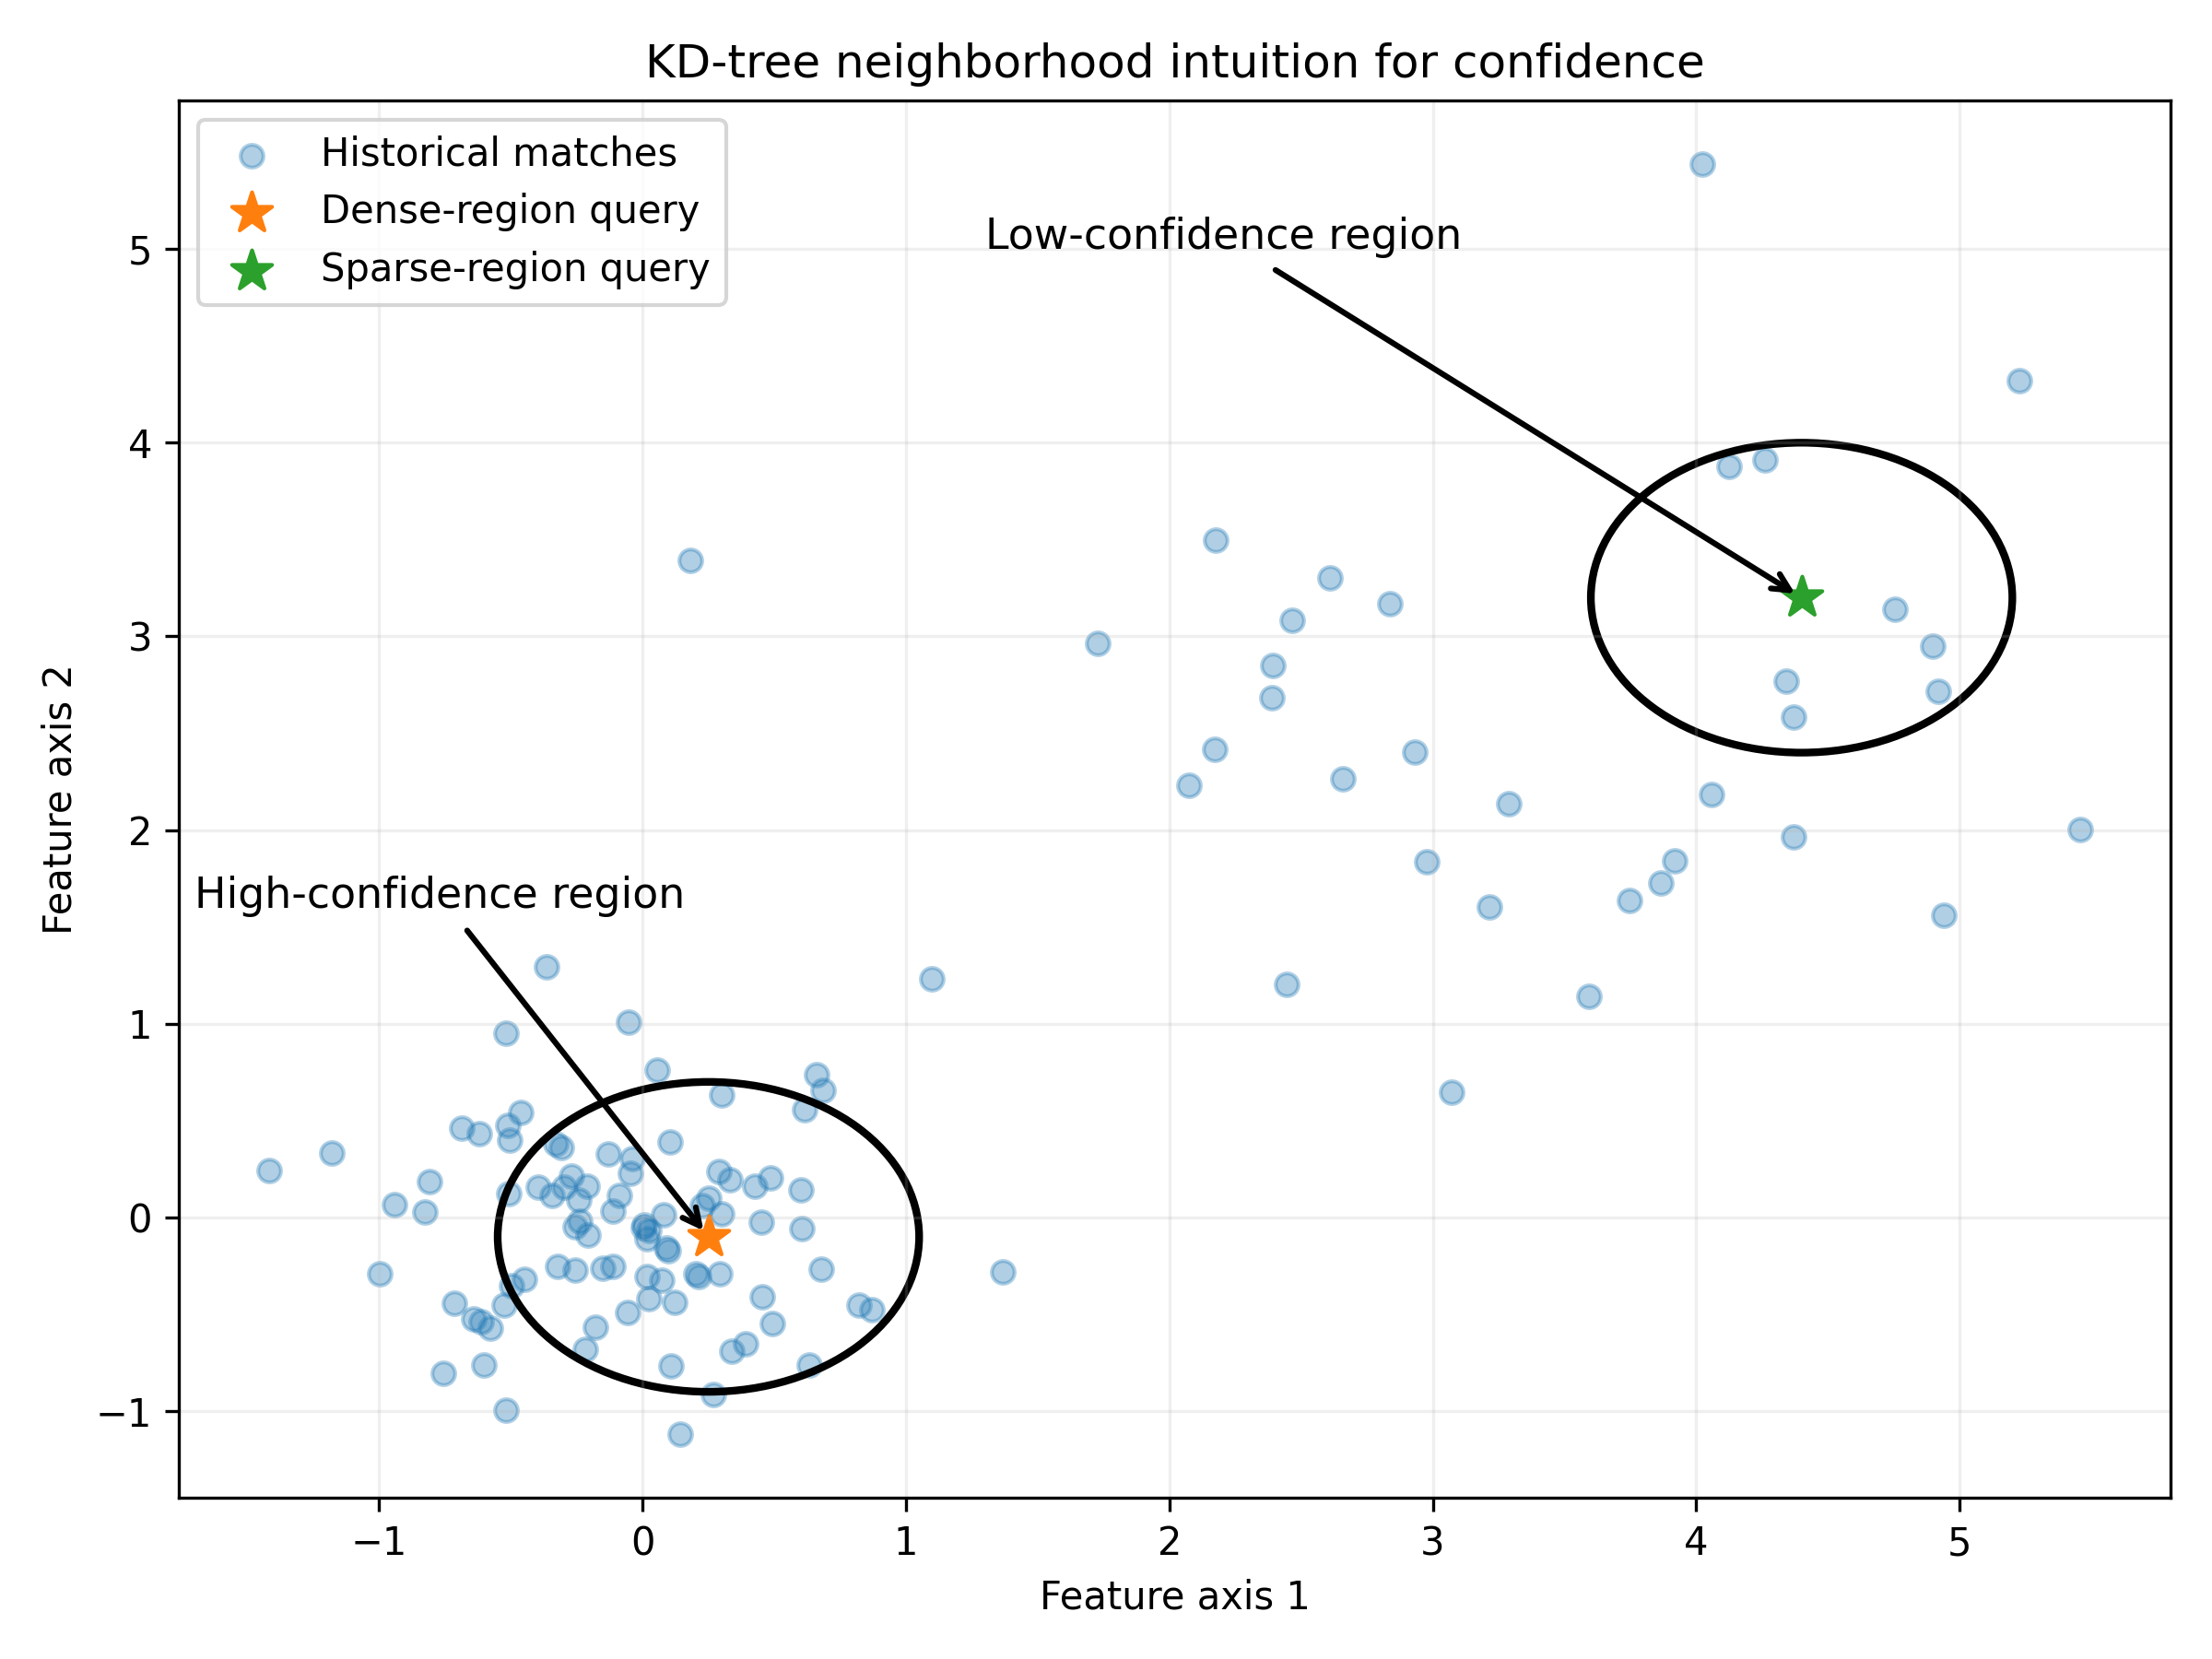
\includegraphics[width=\linewidth]{../poster/poster_images/kdtree_diagram.png}

        \column{0.5\textwidth}
        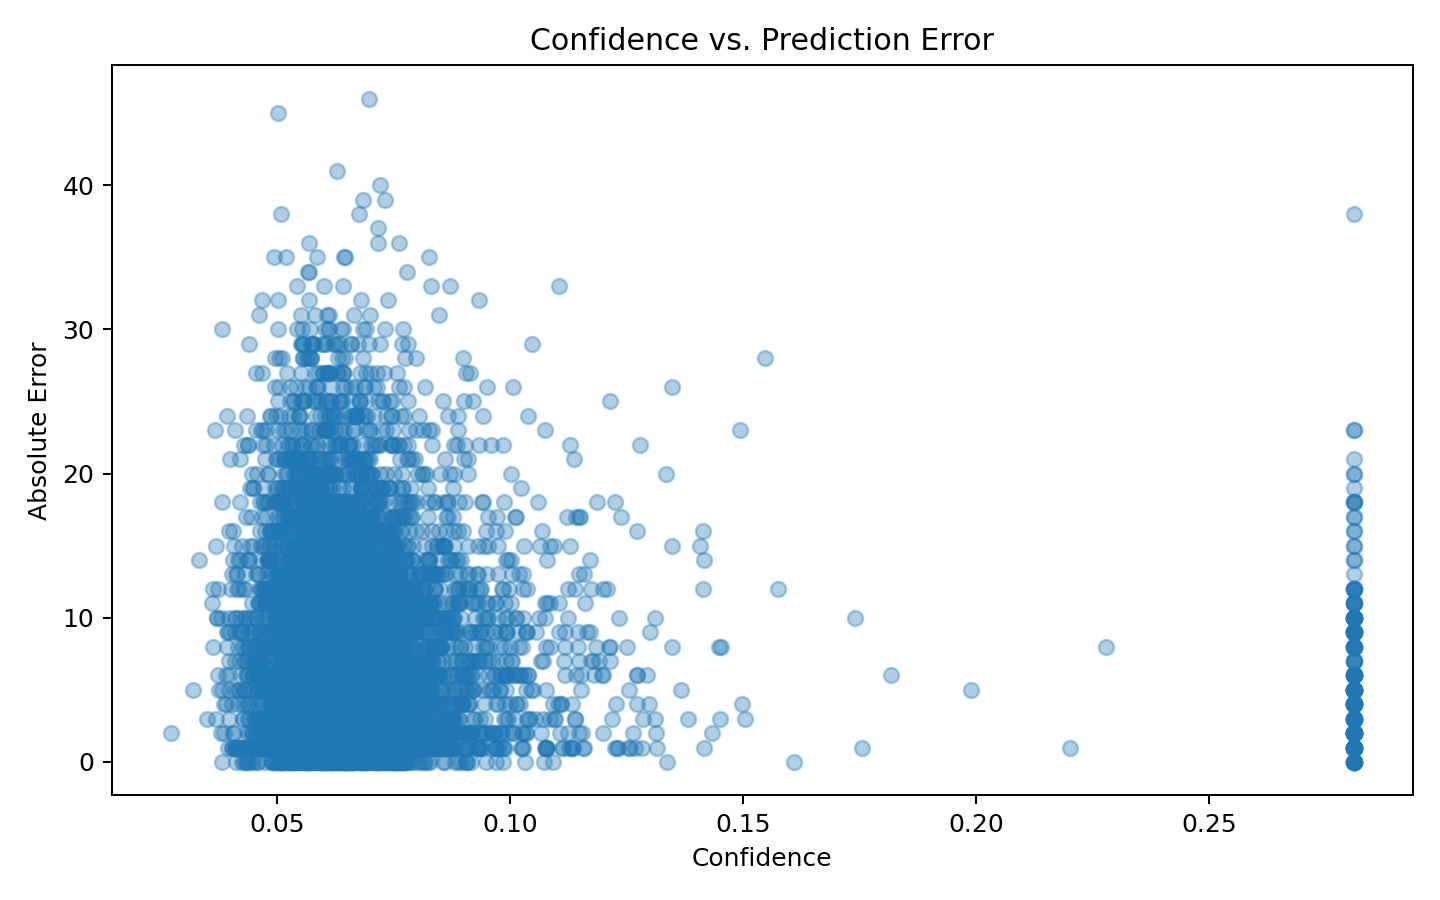
\includegraphics[width=\linewidth]{../paper/figures/confidence_vs_error.png}
    \end{columns}

    \vspace{0.6em}

    \begin{block}{Question}
        Do predictions made in dense regions of feature space have lower error?
    \end{block}

    \begin{itemize}
        \item intuition: dense neighborhoods should imply higher confidence
        \item result: weak relationship for the final nonlinear model
    \end{itemize}
\end{frame}

% =========================================================
\begin{frame}{Conclusion}
    \begin{itemize}
        \item Built a full end-to-end Racketlon prediction pipeline
        \item Dynamic sport-specific ratings provided a strong foundation
        \item Gradient boosted trees gave the best overall performance
        \item Simple KD-tree confidence measures were not very effective for the final model
    \end{itemize}

    \vspace{0.8em}

    \begin{block}{Main lesson}
        The best performance came from combining domain-specific structure with a flexible nonlinear model.
    \end{block}
\end{frame}

% =========================================================
\begin{frame}[plain]
    \begin{center}
        {\Huge Questions?}
    \end{center}
\end{frame}

\end{document}